\documentclass[a4paper,12pt]{article}
\usepackage[utf8]{inputenc}
\usepackage[english]{babel}
\usepackage[T1]{fontenc}
\usepackage{minted}
\usepackage{adigraph}
\usepackage{graphicx}
\usepackage{url}
\usepackage[colorlinks,pdfpagelabels,pdfstartview = FitH,bookmarksopen = true,
bookmarksnumbered = true,linkcolor = black,plainpages = false,hypertexnames = false,
citecolor = black] {hyperref}

\pdfbookmark[1]{tableofcontents}{toc}
\title{Snake-AI\\Project Documentation}
\author{
		Ibrahim Enes Hayber, Rana MD Jewel, Maximilian Lüttich\\
		Frankfurt University of Applied Sciences\\
		Faculty 2, Computer Science (B. Sc.)\\
		Object-oriented Programming in Java by Prof. Dr. Doina Logofatu
}

\date{\today}

\begin{document}

\maketitle
\begin{center}

\includegraphics[scale=0.8]{fra-uas-logo}
\end{center}
\newpage
\tableofcontents

\newpage
\section{How we started}
This chapter describes how we started with the project.\\
\\As we all know the hardest part of a journey is the start. But once started it is a easy on going.
It is like the impact on the first domino stone, which brings the whole project in rolling.
\\As usual in any task of life we need to understand what the problem is and which requirements are necessary to solve the problem. To do so, we read the description from the organizers carefully. In addition to that we watched a few videos about our topic to get a better understanding.\\
After gaining knowledge about the problem we felt ready to start working with the Snake-AI framework, provided by the organizers on a GitHub repository. The framework was written in the Java programming language. To get familiar we looked into the UML class
diagram. Besides that we followed a YouTube Tutorial which was also provided by the organizers, where we implemented our first working version. A detailed introduction and our results will now be presented.
\newpage

\section{Introduction}
Many people know the popular game "Snake" which appeared on a Nokia device back in 1997.
This project focuses on reestablishing Snake but in a different way. 
The most special is that instead moving one single snake manually, we will have two intelligent Snake bots competing against each other.
The aim of a bot is to be the last standing snake or have the highest score by eating apples in 3 minutes. 
\textit{Survival of the fittest} is a great saying.\\
This chapter focuses on the general overview of this project and comparison to similar problems in practice.
\subsection{General Topic}
Our main objective is to make two efficiently working Snake Bots. To create a working bot, all we have to do is to implement a class that implements the Bot interface. This interface has one method which is the \textit{chooseDirection()} method. We can say that the method simulates the brain of the bot. The return value of this method is the direction in which the snake should move to. For directions we have \textit{up, down, left or right}. For example we could implement a first simple bot that just turns right one time. But this type of bot is really uninteresting. For our project we are aiming to implement a bot that uses alogrithms from the fields of Artificial Intelligence. But for now let us look into the game rules.\\
\\The rules are described as follows: \\
\textbf{Rule 1:}  A bot controls only the direction (going either north, south, east, or west) to
be taken by its own snake.\\
\textbf{Rule 2:} Snakes always move simultaneously and forward. Their size increases by one position
(i.e. pixel) after taking an apple.\\
\textbf{Rule 3:} A Snake loses in any of these conditions:\\
\begin{enumerate}
\item If it leaves the board;
\item If it hits its own body;
\item If it hits the other snake's body;
\item If it takes more than one second to make a decision (i.e. which direction to take).
\end{enumerate}
\textbf{Rule 4:} If snakes collide head to head, the longest snake wins the game.\\
\textbf{Rule 5:} Apples appear randomly at an unoccupied position of the board, and there is only
one apple available at any time.\\
\textbf{Rule 6:} An apple will disappear if it is not eaten by either snake in 10 seconds and reappear
somewhere else on the map.\\
\textbf{Rule 7:} At the end of the tournament, players are ranked according to the number of
victories; then the number of draws; then the result of\\

\subsection{Similar problems in practice (References every time, look for actual ones)}
Furthermore, since our bot should be smart then it definetly should use intelligent algorithms. What if we could implement a simple bot that just goes into the direction of the apple and gets closer and closer after every decision. But would this be enough to call it a smart bot? Of course not. Well it is a good behaviour that our snake goes for apples.  But thats not enough. It should also take the shortest path to the apple. For this we want to use algorithm of dijkstra. Dijkstra algorithm is a graph based algorithm which calculates the shortest path from one node to every other node. Let us get a better understanding of this by looking into an example.\\
\\
\NewAdigraph{mygraph}
{
A,blue:0,0;
B:2,0;
C:2,2;
D:0,2;
E,blue:1,3.4
}
{
A,B:12;
B,C:4;
C,A:7; 
A,D, red :1;
D,E, red :2; 
E,C:5;
C,D:9;
}[-]
\mygraph{}
\\
\\We want to know the shortest path from node A to node B. We as human can easily look into that graph and see that taking the route from A-D with cost of 1 is much lesser than rather taking A-C with cost of 7 or A-B with cost of 12. As next we would also see that we have a cost of 2 from D-E. So in total we see that the shortest path from A to D is A-D-E. But telling this to a computer which only knows 0's and 1's is nonsense. Thats why we have algorithms like Dijkstra, which calculates and erases paths with higher costs and returns us the shortest path. Anyway there are many daily life problems where we are using algorithms to compute the shortest path. For example when you are using a navigation tool to drive from one city to an other city. We all would have serious problems if the navigation would take any random path to our destination rather than taking the shortest path or the path with less travel time. Or even when you are crossing over a street where cars are driving. You surely want to take the shortest and safest walkway to the other side.\\
\\Well thats not the only use case of dijkstra in real life applications. When we talk about computer networks we will see a use case of dijkstra too. Considering IP routing to find the shortest path between source and destination router. Dijkstra algorithm is common ly used in routing protocols for updating the forwarding tables.\\
\\Even many dating or social media applications are using dijkstra to recommend you a person which you may know or be interested in. The users can be seen as nodes. The distance could be defined on different aspects like common friends, same interest or even living in the same city.\\
\\A really interesting real life application would be that we could use pathing algorithms in case of emergency calls. If there is a fire anywhere and a emergency call was send out. The algorithm could calculate based on the location which firefighter department is the closest one. Based on this they could send out firefighters. The same could be used for police department and hospitals.

\section{Team Work}
to-do
\subsection{Work Participation}
to-do

\subsection{work structure (communication, decisions, bug tracking, repository, engineering, ...)}
to-do

\subsection{ideas (brainstorming)}
to-do

\section{Problem Description}
to-do
\subsection{Formal description: definitions, examples, ...}
to-do

\section{Related Work}
to-do
\subsection{Related Algorithms, Applications}
to-do

!for example: Fractals, Data Generation, Games, Evolutionary Algorithms (Genetic Algortihms; Collective Intelligence like Particle Swarm Optimization - PSO, Ant Colony Optimizaton - ACO; Evolutionary Multiobjective Optimization, ...)

\section{Proposed Approaches}
to-do
\subsection{Input/Output Format, Benchmarks (Generation, Examples)}
to-do
\subsection{Algorithms in Pseudocode}
to-do

\section{Implementation Details}
 this is my test
to-do
\subsection{Application Structure}
The Snake AI project consists of one Interface, one Enum and eight classes. They are following, 

\begin{itemize}
\item Bot(Interface)
\item Direction(Enum)
\item BotLoader
\item Coordinate
\item Snake
\item SnakeGame
\item SnakeCanvas
\item SnakesRunner
\item SnakeUIMain
\item SnakesWindow
\end{itemize}

\subsection{GUI Details}
In this section all the classes will be discussed in details. 
\subsubsection{SnakeUIMain}
This class is the Entry point of the UI and implements tournament of the Snake game with several rounds. The main method of the class gets two classes(snake \& opponent) implementing the Bot interface as arguments. The class is also responsible to launch several rounds of snake game between bots. In this class the basic I/O actions are performed to record scores of opponent, apple eaten by both the snakes and time taken in each rounds which will be later used to make further statistical analysis.
\subsubsection{BotLoader}
The class BoatLoader fetches the class given the name  of the class and package. The class is taken from the classpath and could be dynamically added after the game of the Bot class. This class inharites the abstrack Java class ClassLoader.\\
A class loader is an object that is responsible for loading classes. The class ClassLoader is an abstract class. Given the binary name of a class, a class loader should attempt to locate or generate data that constitutes a definition for the class. A typical strategy is to transform the name into a file name and then read a "class file" of that name from a file system.%\cite{shafiei2012modeling to-do}
(to-do code snippet)
\begin{minted}{java}
public class BotLoader extends ClassLoader {
    public Class<? extends Bot> getBotClass(String classBinName) {
        try {
            // Create a new JavaClassLoader
            ClassLoader classLoader = Thread.currentThread().getContextClassLoader();

            // Load the target class using its binary name
            Class<?> loadedMyClass = classLoader.loadClass(classBinName);
            boolean isBot = Arrays.asList(loadedMyClass.getInterfaces()).contains(Bot.class);
            if (isBot) {
                System.out.println("Loaded bot.");
            } else {
                System.out.println("Did not match interface.");
            }
            System.out.println("Loaded class name: " + loadedMyClass.getName());

            Class<? extends Bot> botClass = loadedMyClass.asSubclass(Bot.class);
            Constructor<? extends Bot> botClassCtor = botClass.getConstructor();
            return botClass;

        } catch (Exception e) {
            e.printStackTrace();
        }

        return null;
    }
}

\end{minted}
\\
The only method of BotLoader class gets classBinName as argument and returns an instance of the Bot class.

\subsubsection{SnakesWindow}
This class is responsible for the game's GUI window. The class creates and set ups the window and runs the UI. At the end it closes the frame. This class implements Runnable.\\
The Runnable interface should be implemented by any class whose instances are intended to be executed by a thread. The class must define a method of no arguments called run.\\
This interface is designed to provide a common protocol for objects that wish to execute code while they are active. For example, Runnable is implemented by class Thread.
 Being active simply means that a thread has been started and has not yet been stopped.\\
In addition, Runnable provides the means for a class to be active while not subclassing Thread. A class that implements Runnable can run without subclassing Thread by instantiating a 
Thread instance and passing itself in as the target. In most cases, the Runnable interface should be used if you are only planning to override the run() method and no other Thread methods. This is important because classes should not be subclassed unless the programmer intends on modifying or enhancing the fundamental behavior of the class.(to-do ref)
\subsubsection{SnakesRunner}
This class also implements Runnable interface and is used for running bots in a separate threads. The Constructor of the class SnakesRunner recieves running bot, snake that is controlled by the current bot, opponent's snake, size of the board and coordinate of the current apple as arguments. In addition the chooseDirection method of the current bot is executed and saved(current direction) by this class. 
\subsubsection{SnakesGame}
The class SnakesGame implements the main games flow and runs game for two bots. The Override toString() method converts the game to string representation and return game state as a string. randomNonOccupiedCell() method selects random non-occupied cell of maze which is used to create new location of a apple. If a Snake takes more than one seconds to choose its  next direction the runOneStep() methods stopps that rounds.

\subsubsection{SnakeCanvas}
The purpose of this class is to design the UI and give the UI a better look. This class helps to fill the  snake Body wicht color and make it visible on the UI. After filling the body of snake and opponent and apple the render() method renders the game. After every movement of the snake, opponent and apple the previous occupied positions are recolord and marked the free for next movement. This class inharites the Java swing class JPanel which is used to create different generic lightweight container with one or more single component.
\subsubsection{Snake}
This class implements snake body(not brain) that determines the place of head, body, and length of body on the game board. For implementing the body of the snake two logical and efficient data structure from Java Collections framework are used. They are,
\begin{itemize}
\item Dequeue
\item HashSet
\end{itemize}
Deque(double ended queue) data structure helps to add or delete elements from both side(head and tail) within $\mathcal{O}(1)$ constant time coplexity. On the other hand HashSet data structure ensures basics search operation in $\mathcal{O}(1)$ time complexity.\\
This class has a important feature of cloneability which allows to copy one object to another object without using new operator.\\
A class implements the Cloneable interface to indicate to the Object.clone() method that it is legal for that method to make a field-for-field copy of instances of that class.
Invoking Object's clone method on an instance that does not implement the Cloneable interface results in the exception CloneNotSupportedException being thrown.(to-do ref)
\subsubsection{Coordinate}
Coordinates class implements position of a cell on the game board. It helps to grow up the snake by adding new coordinate at the beginning of the snake body. inBounds() methods helps to keep the snake in side the game board. This methods implements Comparable interface which is useful while comparing two Coordinate. 
\subsubsection{Bot}
This Interface provides functions that should be implemented to create smart and intelligent snake bot for the game. chooseDirection() methds returns an appropriate next moves which plays a vital role to continue the game. 

\subsection{UML Diagram}

\begin{figure}[h]
\centering
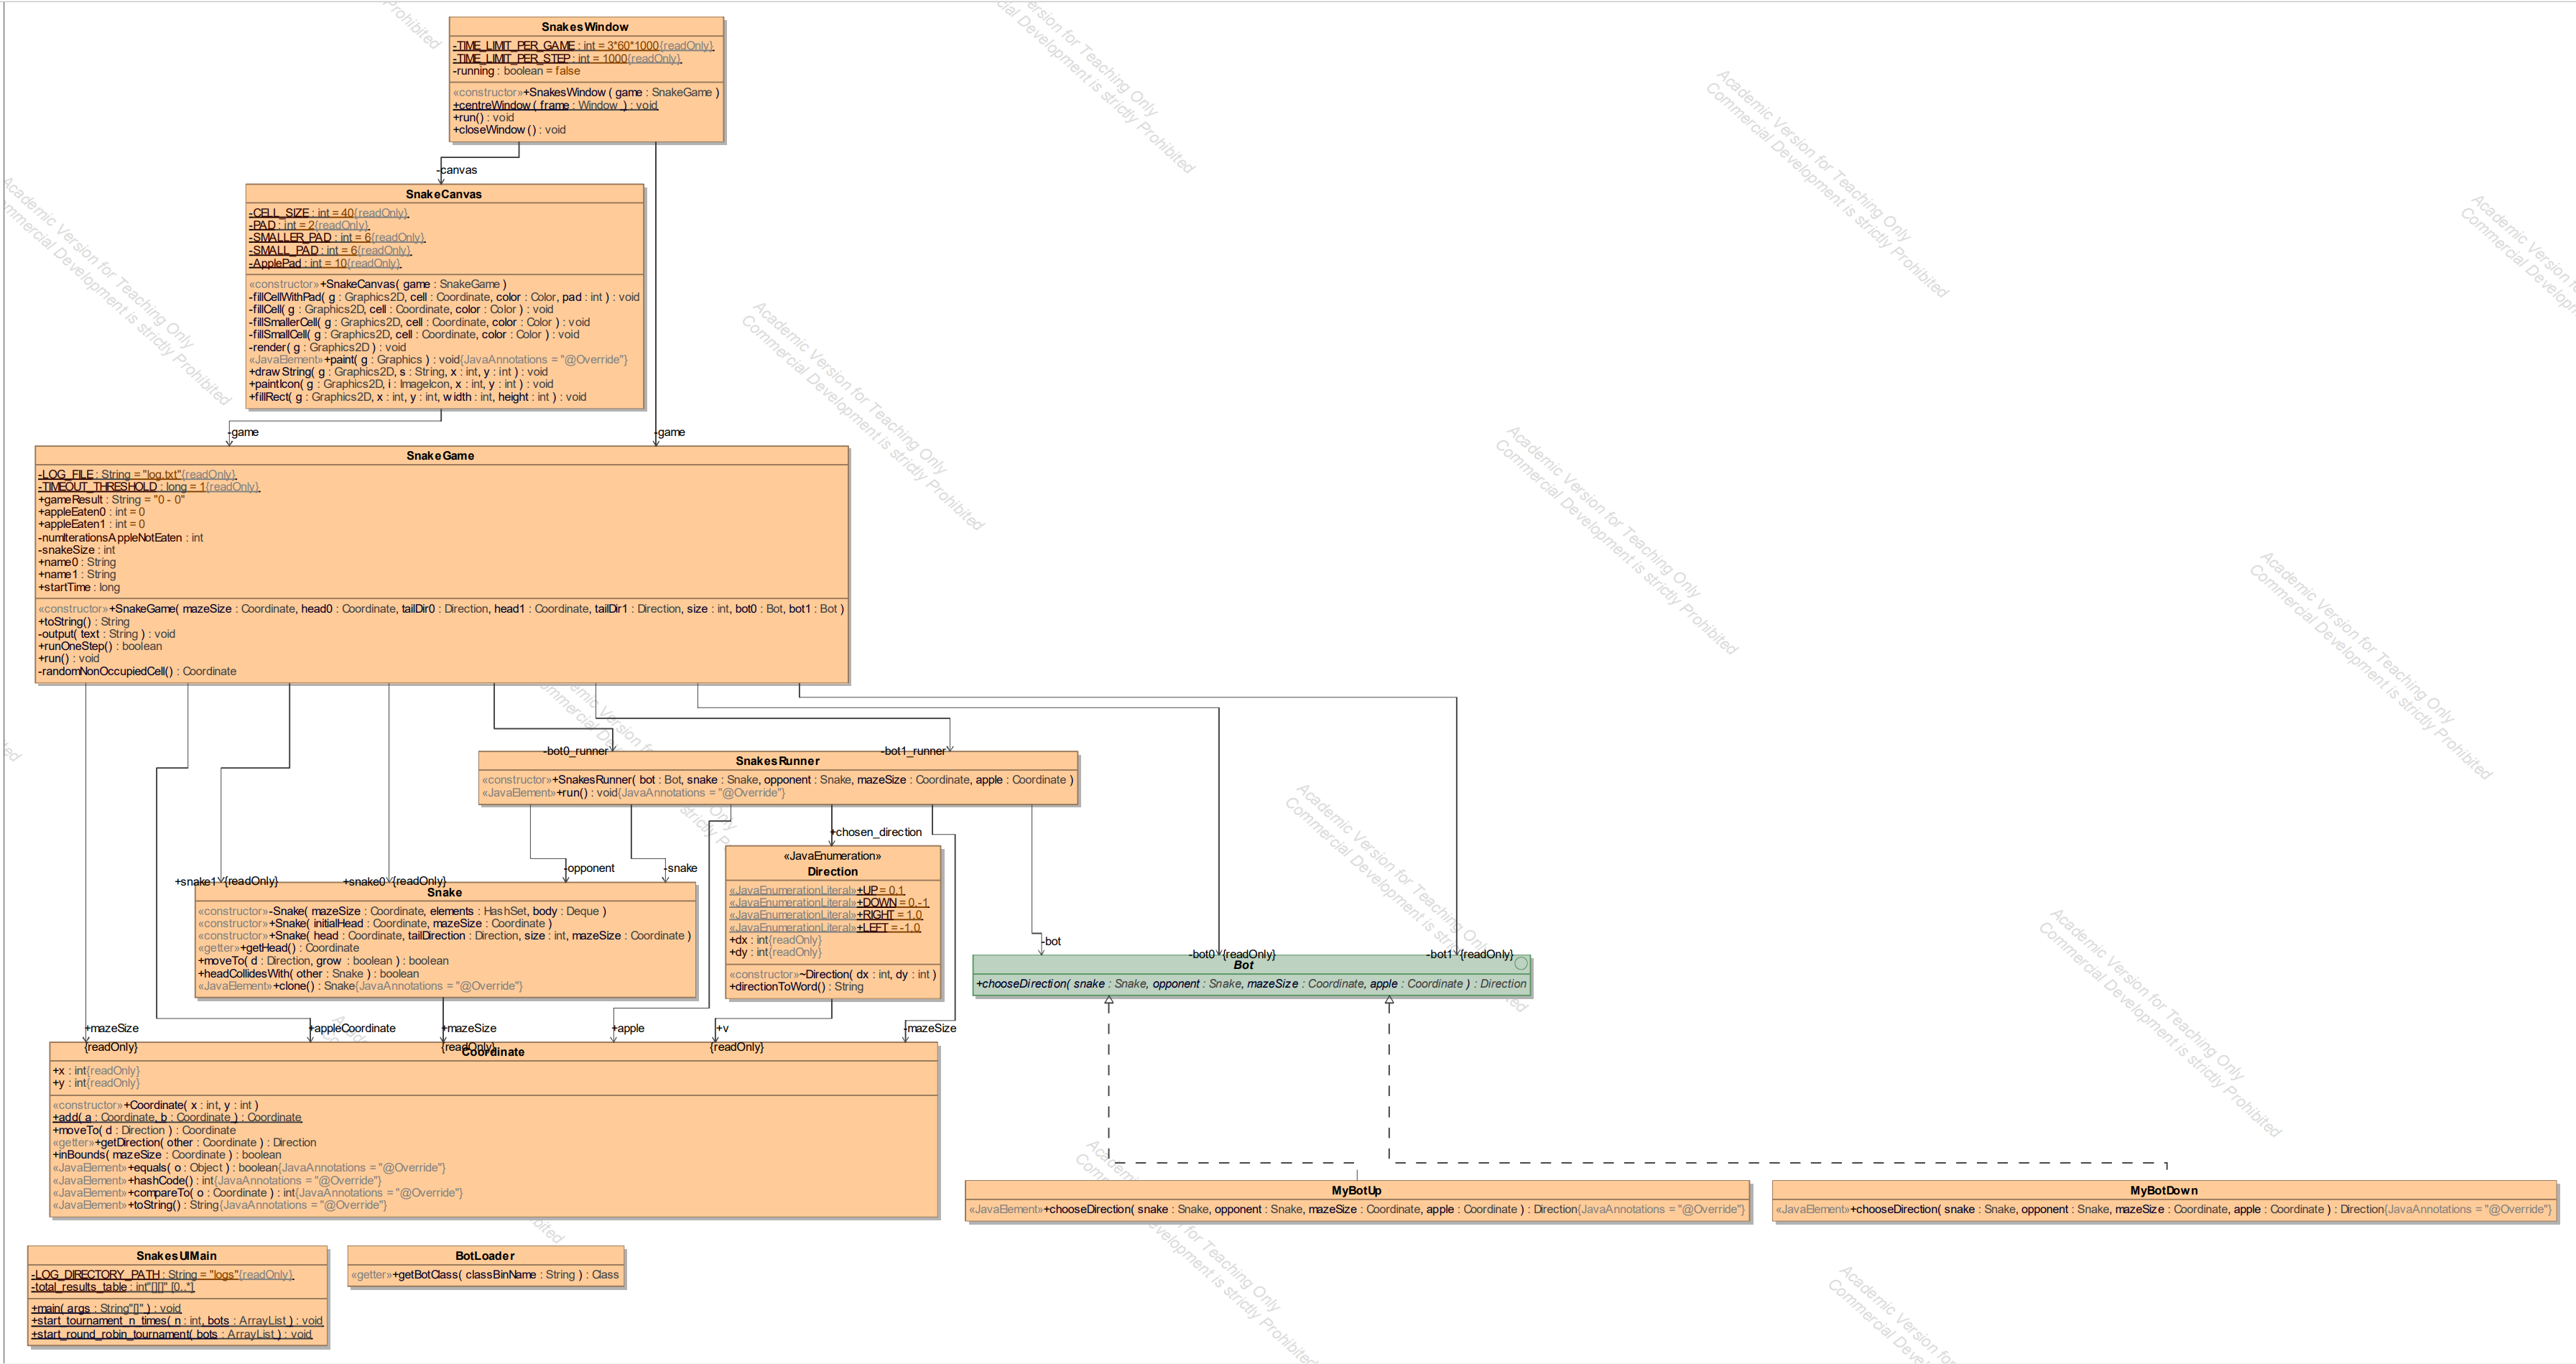
\includegraphics[scale=0.26]{ui.png}
\caption{UML diagram of the GUI}
%\label{fig:abc}
\end{figure}

\subsection{Used Libraries}
For the Developement of the Snake AI Game Java Swing Framework has been used.
Some Components from AWT framework have also been used.\\ 
Swing is a Java Foundation Classes [JFC] library and an extension of the Abstract Window Toolkit [AWT]. Swing offers much-improved functionality over AWT, new components, expanded components features, and excellent event handling with drag-and-drop support.(to-do ref)
 
%\subsection{Code Snippets} write code snippet with discription.
\subsection{Bot1}
\title{Bot 1 (IntBot1.java):}\\
\\
After getting to know the framework of our task, one of our first objectives was implementing a
basic bot by ourselves that does the following:\\
\begin{itemize}
\item Calculate all valid moves
\item Exhibit a basic avoidance behavior regarding the opponent
\item Go for the apple
\end{itemize}
This basic bot also served as an opponent for more advanced bots later on.\\
\\
To keep things organized, we decided to create a package for each bot. The packages were created
in the „src“-folder of the given project. Each bot consists of a public class that implements the
Interface „Bot“, which as previously described, consists of only one method: „chooseDirection“.
Properly overriding this method turned this class into a bot that could be used in the game.
\\
\\
The basic idea for creating this bot was that a static array that contains all possible directions
(Direction.RIGHT, Direction.DOWN, Direction.UP, Direction.LEFT) is created outside the method
„chooseDirection“ and inside the method each element of this array is checked for its worth
concerning the stated objectives. This concept was also used in the provided example of  a bot  on the following website: \url{https://github.com/BeLuckyDaf/snakes-game-tutorial} The only thing that this bot was concerned with was not killing itself.\\
\\
Creating the static array:
\begin{minted}{java}
public class IntBot1 implements Bot {
private static final Direction[] DIRECTIONS = new Direction[]{Direction.RIGHT,
Direction.DOWN, Direction.UP, Direction.LEFT};
@Override
public Direction chooseDirection(Snake snake, Snake opponent, Coordinate
mazeSize, Coordinate apple) {
\end{minted}
The first thing we did was to create an array of possible directions of the opponent’s head and a set
that contains the resulting coordinates, so that at the end of the method „chooseDirection“ the
coordinates could be removed from the pool of possible directions of our bot’s head. To create such
an array, it was necessary to determine the coordinate of the second element of the opponent snake.
We used an iterator to achieve this in the following way:\\
\begin{minted}{java}
//Position of second Element of opponent
Coordinate afterHeadNotFinal2 = null;
if(opponent.body.size()>=2){
Iterator<Coordinate> it = opponent.body.iterator();
it.next();
afterHeadNotFinal2 = it.next();
}
final Coordinate afterHead2 = afterHeadNotFinal2;
//second element of opponent snake
\end{minted}
Note that the class „Snake“ featured a deque of elements of the „Coordinate“-class called „body“.\\
\\
After that, we used a stream method to get a sequential stream of the elements from the array
„DIRECTIONS“ to create a new array of directions called „validMovesOpponent“. The direction
whose result would equal the second element of the opponent snake was filtered out using the “equals”-method on coordinate objects. Finally, a Set of coordinates called
“possiblePositionsOpponent” was created by simply using the “moveTo” method on the head of the
opponent snake and having all elements of “validMovesOpponent” as parameters.
\begin{minted}{java}
Direction[] validMovesOpponent = Arrays.stream(DIRECTIONS)
.filter(d -> !head2.moveTo(d).equals(afterHead2))
.sorted()
.toArray(Direction[]::new);
Set<Coordinate> possiblePositionsOpponent = new HashSet<>();
for(int i=0; i< validMovesOpponent.length; i++){
possiblePositionsOpponent.add(head2.moveTo(validMovesOpponent[i]));
}
\end{minted}


Since no other restrictions were made, the set „possiblePositionsOpponent“ always contained three
elements, even if they were to be outside the maze.\\
\\
Analogous to the array „validMovesOpponent“ we created an array of directions called
„validMoves“ for our bot’s snake that excluded the possibility of backwards movement of the
snake. This array „validMoves“ was subsequently used as a parameter of the stream method to
create a new array of directions called „notLosing“, that with the use of the filter method excluded
some unfavorable outcomes.
\begin{minted}{java}
Direction[] notLosing = Arrays.stream(validMoves)
.filter(d -> head.moveTo(d).inBounds(mazeSize))
.filter(d -> !opponent.elements.contains(head.moveTo(d)))
.filter(d -> !snake.elements.contains(head.moveTo(d)))
.filter(d -> !possiblePositionsOpponent.contains(head.moveTo(d)))
.sorted()
.toArray(Direction[]::new);
\end{minted}

Using the filter method, we checked the following: Is the resulting coordinate outside the
maze? Is the resulting coordinate part of the opponent’s body? Is the resulting coordinate
part of our snake’s body? And finally, does the set „possiblePositionsOpponent“ contain the
resulting coordinate? If the answer to each of these question was „no“ the streamed element
was added to the array.\\
\\
Finally, we used the bubble sort algorithm to sort the elements of „notLosing“ based upon
the distance to the apple. „chooseDirection“ returns the first element of „notLosing“
provided that this array is not empty. If this array happens to be empty, the first element of
„validMoves“ is returned which, is never empty.
\begin{minted}{java}
//Bubble Sort; Sorting Elements of "NotLosing"
double distance1, distance2;
int a1, a2, h11, h12, h21, h22, d1, d2;
Coordinate test1, test2;
Direction temp;
if (notLosing.length > 0){
a1=apple.x;
a2=apple.y;
for(int i=0; i< notLosing.length; i++){
for(int a= i+1; a< notLosing.length; a++){
test1 = head.moveTo(notLosing[i]);
test2 = head.moveTo(notLosing[a]);
h11= test1.x;
h12 = test1.y;
d1 = (h11-a1)*(h11-a1)+(h12-a2)*(h12-a2);
distance1=Math.sqrt((double)d1);
h21= test2.x;
h22 = test2.y;
d2 = (h21-a1)*(h21-a1)+(h22-a2)*(h22-a2);
distance2=Math.sqrt((double)d2);
if(distance2<distance1){
temp=notLosing[i];
notLosing[i]=notLosing[a];
notLosing[a]=temp;
}
}
}
return notLosing[0];
}
else{
return validMoves[0];
}
}
\end{minted}
The biggest drawback of this bot was the frequent entrapment with itself or the opponent’s snake. Even though basic evasive movements were often enough to avoid losing the game, more complex dangers like a U-shape of the opponent’s snake or the bot’s snake could not be recognized by this bot. This becomes more apparent the more elements the bodies of the snakes have.\\
\subsection{Bot2}

The idea behind my Bot is the famous Dijkstra Algorithem which is most widely used to find the shortest path.
In my Programm before I give my Snake a Direction first of all I  always choose four adjucent cells from the current
Head position of the Snake. Secondly, I have to eliminate one of the cell from them which is already located in the Snake
body (next Cordinate after the Head). Thirdly, I have been checking whether the given move leads the Snake out of the Maze.
Then with the help of Pythagoras formula I calculate the distance between the next postion of the Snake  and the apple.
After that I calculate the minimum between all the distances. Finally I give the Snake the next Direction.
\begin{minted}{java}
    // functions to evaluate a valid move
    // prevent snake to hit border of the board
    // prevent to avoid collision
    // prevent backward movement
    boolean isValidMove(Snake snake,Coordinate mazeSize,Direction d,
	HashSet<Coordinate>opponentPos,Snake opponent){

        if(snake.getHead().moveTo(d).inBounds(mazeSize) && 
		!snake.elements.contains(snake.getHead().moveTo(d)) && 
        !opponentPos.contains(snake.getHead().moveTo(d)) && 
		!opponent.elements.contains(snake.getHead().moveTo(d))){
            //&& !opponent.elements.contains(snake.getHead().moveTo(d)
            return true;
        }
        return  false;

    }
\end{minted}
But in this Algorithem I was not considering the position of the opponent Snake. As a result there were many collisions between my Snake and opponent 
Snake. To get rid of this I have also figured out all the possible next move of the Opponent Snake and saved them in a HashSet. While giving the next move 
to my Snake I check whether this next move is also the next move of the opponent Snake or not. This has solved the Head to Head collision. But still there were some 
collision with Body of the opponent Snake. That's why I have also justified whether the next move is one of the element of the opponent Body or not.

\begin{minted}{java}
  //variables to find all the distance from next move to apple
        int disFromLeft = Integer.MAX_VALUE, disFromRight=Integer.MAX_VALUE,
		disFromUp=Integer.MAX_VALUE,disFromDown=Integer.MAX_VALUE;

        if (isValidMove(snake, mazeSize, Direction.UP, 
		(HashSet<Coordinate>) possiblePositionsOpponent,opponent)) {

            Coordinate toUp = snake.getHead().moveTo(Direction.UP);
            // find minimum distance from up to the apple using Pythagoras
            disFromUp =(int) Math.sqrt(Math.pow(toUp.x- apple.x,2)+
			Math.pow(toUp.y- apple.y,2));

        }
        if (isValidMove(snake, mazeSize, Direction.LEFT,(HashSet<Coordinate>) 
		     possiblePositionsOpponent,opponent)) {

            Coordinate toLeft = snake.getHead().moveTo(Direction.LEFT);
               // find minimum distance from left to the apple using Pythagoras
            disFromLeft =(int) Math.sqrt(Math.pow(toLeft.x- apple.x,2)+
			       Math.pow(toLeft.y- apple.y,2));

        }
        if (isValidMove(snake, mazeSize, Direction.DOWN,(HashSet<Coordinate>) 
		          possiblePositionsOpponent,opponent)) {

            Coordinate toDown = snake.getHead().moveTo(Direction.DOWN);
             // find minimum distance from down to the apple using Pythagoras
            disFromDown =(int) Math.sqrt(Math.pow(toDown.x- apple.x,2)+
			   Math.pow(toDown.y- apple.y,2));

        }
        if (isValidMove(snake, mazeSize, Direction.RIGHT,(HashSet<Coordinate>)
		      possiblePositionsOpponent,opponent)) {

            Coordinate toRight = snake.getHead().moveTo(Direction.RIGHT);
                   // find minimum distance from right to the apple using Pythagoras
            disFromRight =(int) Math.sqrt(Math.pow(toRight.x- apple.x,2)+
			      Math.pow(toRight.y- apple.y,2));
        }
       // find minimum from all the possible paths
        int minDis = Math.min(Math.min(disFromRight,disFromDown),
		       Math.min(disFromUp,disFromLeft));
            
            //give direction to the snake
        if(minDis==disFromRight){
            return Direction.RIGHT;
        } 
        else if(minDis==disFromDown){

            return Direction.DOWN;
        }
        else if(minDis==disFromLeft){

            return  Direction.LEFT;
        }
        else if(minDis==disFromUp) {
            return Direction.UP;
        }
        else{
          // to avoid worst cases.
            Random rn = new Random();
            int pos = rn.nextInt(3);
            switch (pos){

                case 0:
                    return Direction.RIGHT;
                case 1:
                    return Direction.LEFT;
                case 2:
                    return Direction.UP;
                default:
                    return Direction.DOWN;
            }
        }

\end{minted}
In term of Time and Space Complexity this Algorithem is quite efficient. The Algorithem has Time Complexity of O(1) and Space
Complexity is approximately O(n). Wher n is the number of elements of Opponent Snake body. 

Inspite of all the Consideration there is still some Collisions in critical Situation. Anothe problem is Self Entrapping. 

\subsection{Bot3}

\section{Experimental Results and Statistical Tests}
to-do
\subsection{Simulations (Play with the Parameters!)}
to-do
\subsection{Use Benchmarks}
to-do
\subsection{Tables: input data details, results of different algorithms}
to-do
\subsection{Charts}
to-do
\subsection{Evaluations}
to-do

\section{Conclusions and Future Work}
to-do
\subsection{How the team work went}
to-do
\subsection{What we have learned}
to-do
\subsection{Ideas for the future development of your application, new algorithms}
to-do

hello world
\end{document}